\documentclass[12pt,a4paper]{article}

\usepackage[utf8]{inputenc}
\usepackage{amsmath}
\usepackage{graphicx}
\usepackage{hyperref}
\usepackage{geometry}
\usepackage{float}
\geometry{margin=1in}

\title{numberAI: Building an Image Classifier from Scratch}
\author{Project Documentation}
\date{\today}

\begin{document}

\maketitle

\begin{abstract}
This document outlines the development, architecture, and findings of the \textbf{numberAI} project. The objective of this project is to recreate machine learning functionality from scratch, without relying on pre-trained models or established neural network structures. By utilizing simple matrix multiplication and a trial-and-error training approach, the project aims to categorize number images. Additionally, it details the planned second phase involving quantization and distillation for deployment on resource-constrained embedded systems such as Arduino.
\end{abstract}

\tableofcontents
\newpage

\section{Introduction}
\subsection{Project Motivation}
Modern machine learning often relies on complex, pre-defined architectures and pre-trained weights. The motivation behind numberAI is to deconstruct this paradigm and build an image classifier from the absolute basics to fully understand the underlying mechanics of neural networks.

\subsection{Goals and Phases}
The project is divided into two main phases:
\begin{itemize}
    \item \textbf{Phase 1: Foundational Discovery.} To categorize number images using pure matrix multiplication. This phase avoids pre-defined structures, instead relying on trial and error to iteratively discover the optimal matrix size and network topology.
    \item \textbf{Phase 2: Embedded Systems Deployment.} To run the developed classification model on embedded systems with limited resources (e.g., Arduino). This requires applying model compression techniques such as \textit{quantization} and \textit{distillation} to reduce memory footprint and computational load.
\end{itemize}

\section{System Architecture}
The system architecture of numberAI is built upon a custom pipeline designed to handle raw images, process them into matrices, apply matrix multiplication, and verify the outputs. 

\begin{figure}[H]
    \centering
    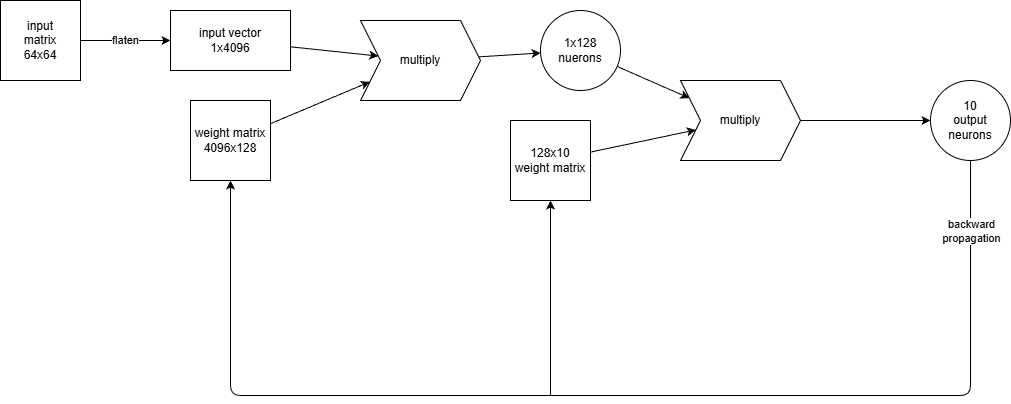
\includegraphics[width=0.8\textwidth]{./image/architecturev1.png}
    \caption{System Architecture of numberAI}
    \label{fig:architecture}
\end{figure}


\subsection{Data Processing Pipeline}
The input processing pipeline involves converting raw number images into a format suitable for matrix multiplication. 
% TODO: Elaborate on the specific image preprocessing steps (e.g., grayscaling, normalizing).
The script \texttt{image2txt.py} is responsible for converting input images (stored in \texttt{inputImage}) into a text-based matrix representation (stored in \texttt{inputText}). These processed inputs are then matched against their corresponding expected outputs (stored in \texttt{expectedAnswer}).

\subsection{Model Structure (Hidden Layers)}
Instead of a fixed neural network topology, the model's architecture is dynamic. The structure consists of customizable hidden layers whose weights and biases are stored in the \texttt{hiddenLayer} directory. The exact dimensions of these matrices are subject to experimentation and tuning during the training phase.

\section{Methodology}
\subsection{Inference (Forward Pass)}
The core inference logic is implemented in \texttt{run\_model.py}. The process relies purely on sequential matrix multiplications of the input text data with the matrices defined in the hidden layers to yield a final categorization prediction.

\subsection{Training via Trial and Error}
Unlike traditional backpropagation implementations, the training process handled by \texttt{train\_model.py} employs a numerical gradient estimation approach, often framed as trial-and-error. 

The loss function used to evaluate the model's performance calculates the sum of the Euclidean distances between the actual output vector ($\mathbf{A}$) and the expected output vector ($\mathbf{EA}$) across all 10 training samples:
\begin{equation}
\mathbf{Loss} = \sum_{k=0}^{9} \sqrt{\sum_{n=0}^{9} \left( A_{k,n} - EA_{k,n} \right)^2}
\end{equation}
Where $A_{k}$ is the length-10 output vector for the $k$-th input number image, and $EA_{k}$ is the corresponding expected answer.

To adjust the weights and decrease the loss, the algorithm perturbs a specific weight (e.g., $H1_{m,n}$) by a small \textit{change} and observes the new loss ($\mathbf{Loss}_{o+\text{change}}$). The weight is then updated using the numerical gradient approximation:
\begin{equation}
H_{m,n} := H_{m,n} - \left( \frac{\mathbf{Loss}_{o+\text{change}} - \mathbf{Loss}_{o}}{\text{change}} \right) \cdot \alpha
\end{equation}
Where $\mathbf{Loss}_{o}$ is the original loss, and the learning rate $\alpha$ is scaled proportionally to the loss. This heuristic method bypasses complex calculus by explicitly calculating the finite difference to approximate the derivative.

\subsection{Model Reset}
To facilitate repeated experimentation, \texttt{reset\_model.py} provides the functionality to re-initialize the matrix weights using random uniform distributions (\texttt{np.random.rand}). This allows the trial-and-error process to start fresh from different initial states.

Upon resetting the two primary hidden layers (\texttt{H1} of size $256 \times 32$ and \texttt{H2} of size $32 \times 10$), the initial Shannon entropy of the randomly generated weights was recorded to establish a baseline before training:
\begin{itemize}
    \item \textbf{H1 Entropy:} 6.633968859734219
    \item \textbf{H2 Entropy:} 6.45341914045563
\end{itemize}
Tracking this entropy provides insight into the information density and randomness of the network before it adapts through trial-and-error iterations.

\section{Architecture Iterations}
As the project employs a trial-and-error discovery method, the model architecture is expected to evolve through multiple versions as optimal matrix sizes and structures are found.

\subsection{Version 1.0 Architecture}
The initial structure (\textbf{Version 1.0}) consists of the following components:
\begin{itemize}
    \item \textbf{Input Layer}: Flattened representation of the input image.
    \item \textbf{Hidden Layers}: Two primary weight matrices ($H1$ and $H2$), where dimensions were iteratively tested (e.g., $256 \times 32 \to 32 \times 10$, and later $4096 \times 128 \to 128 \times 10$).
    \item \textbf{Output Layer}: Vector of size $10 \times 1$, representing the classification scores for digits 0-9.
\end{itemize}

\subsubsection{Version 1.0 Training Results}
After training the Version 1.0 architecture via the numerical gradient approach, a measurable drop in Shannon entropy for the weight matrices was observed:
\begin{itemize}
    \item \textbf{Pre-training Entropy}: $H1 \approx 6.63$, $H2 \approx 6.45$
    \item \textbf{Post-training Entropy}: $H1 \approx 3.05$, $H2 \approx 3.23$
\end{itemize}
This lower entropy strongly indicates that the trial-and-error process successfully converged on structured patterns within the dataset rather than remaining random. A visualization of the training loss can be seen below:

\begin{figure}[H]
    \centering
    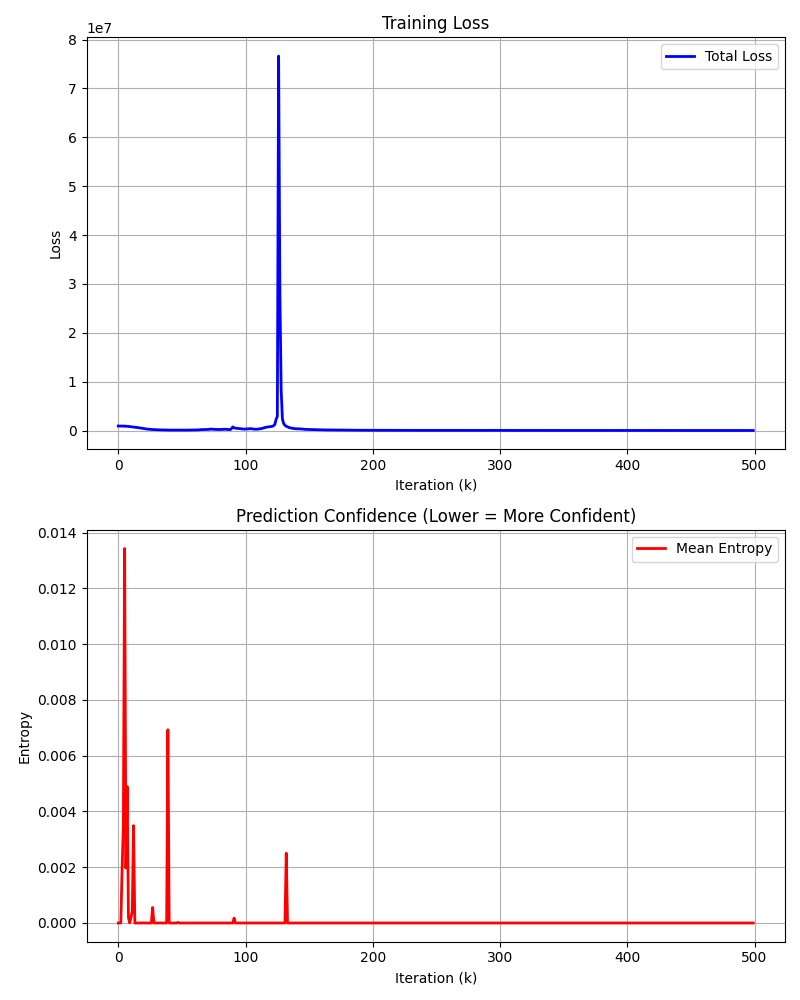
\includegraphics[width=0.8\textwidth]{./image/trainV1.png}
    \caption{Version 1.0 Training Loss Progression}
    \label{fig:trainV1}
\end{figure}

\subsection{Version 2.0 Architecture (Planned)}
% TODO: Document Version 2.0 changes (e.g., new matrix sizes, added activation functions, changes in topology) once implemented.
[Placeholder: Describe changes made in Version 2.0 to improve upon the shortcomings of Version 1.0. For example, adjusting matrix sizes or altering the pipeline to fix accuracy bottlenecks.]

\section{Phase 2: Embedded Systems Optimization}
% TODO: Fill in the findings once Phase 2 is underway.
To deploy this model on an Arduino, the network must be significantly compressed.
\subsection{Quantization}
[Placeholder: Describe the process of converting floating-point matrix weights to lower precision formats (e.g., 8-bit integers) and the resulting impact on accuracy.]

\subsection{Distillation}
[Placeholder: Describe how a smaller, more efficient model (student) is trained to replicate the behavior of the larger, successful trial-and-error model (teacher).]

\section{Discoveries and Challenges}
% TODO: Document any new findings, discoveries, or reasons for failure during the trial and error process.
\subsection{Matrix Size Optimization}
[Placeholder: Discuss which matrix dimensions yielded the best balance between accuracy and computational complexity.]

\subsection{Trial and Error Efficiency}
[Placeholder: Discuss the challenges faced when training without traditional gradient descent. What heuristics were discovered to speed up convergence?]

\section{Conclusion}
[Placeholder: Summarize the final outcomes of the project, whether the goals were fully met, and potential future improvements.]

\end{document}
